\themaG
\graphicspath{{../Ch21_Les_quadrilateres/Images/}}

\chapter{Les quadrilatères}
\label{C24}


%%%%%%%%%%%%%%%%%%%%%%%%%%%%%%%%%%%%%%%%%%
\begin{prerequis}[Connaissances et compétences abordées]
   \begin{itemize}
      \item Reconnaître, nommer, décrire des quadrilatères, dont les quadrilatères particuliers (carré, rectangle, losange, première approche du parallélogramme).
      \item Vocabulaire associé à ces objets et à leurs propriétés : côté, sommet, angle, diagonale, polygone.
   \end{itemize}
\end{prerequis}

\vfill

\begin{debat}[Débat : vocabulaire des quadrilatères]
   Le mot {\bf quadrilatère} provient du latin : {\it quatuor}, quatre, et {\it latus}, côté. Il existe un mot équivalent d'origine grecque : {\bf tétrapleure} de {\it tèssera}, quatre, et {\it pleura}, côté ou {\bf tétragone}, de {\it gônia}, angle. \\
   Comme pour les triangles, les quadrilatères peuvent être particuliers selon qu'ils ont certaines propriétés : parmi ceux-ci, on peut trouver par exemple la famille des trapèzes, des parallélogrammes, des rectangles, des losanges, des carrés ou encore des cerfs-volant. \\
   \begin{center}
      {\psset{unit=0.7}
      \begin{pspicture}(-1,-0.5)(14,7.5)
         \psframe[linecolor=red](7.25,0.25)(9.75,7.5)
         \psframe[linecolor=yellow](0.5,0.5)(9.5,2.5)
         \psframe[linecolor=orange](4.25,0)(10,5)
         \psframe[linecolor=orange!50](0.25,-0.25)(10.25,5.25)
         \psframe[linecolor=red!50](0,-0.5)(10.5,7.75)
         \psframe[linecolor=blue](-0.25,-0.75)(13.75,8)
         \psset{fillstyle=solid}
         \psframe[fillcolor=yellow](8,1)(9,2) %carré
         \psframe[fillcolor=yellow!50](5,1)(7,2) %rectangle
         \pspolygon[fillcolor=yellow!25](1,1)(3,1)(3,2)(1.5,2) %trapèze rectangle
         \pspolygon[fillcolor=orange!25](1,3.5)(3.5,3.5)(2.5,4.5)(1.5,4.5) %trapèze
         \pspolygon[fillcolor=orange!50](4.5,3.5)(6.25,3.5)(6.75,4.5)(5,4.5) %parallélogramme
         \pspolygon[fillcolor=orange](7.5,4)(8.5,3.5)(9.5,4)(8.5,4.5) %losange
         \pspolygon[fillcolor=red!50](3,6.5)(3,7)(5,7.5)(4.5,6) %convexe
         \pspolygon[fillcolor=red](8,6.75)(8.5,7.25)(9,6.75)(8.5,5.5) %cerf-volant
         \pspolygon[fillcolor=cyan!50](11,1.5)(13.5,3)(13,1.5)(11.25,2.5) %croisé
         \pspolygon[fillcolor=cyan](11,5)(13,5)(12.5,7)(12,5.5) %concave
      \end{pspicture}}
   \end{center}
   \bigskip
   \begin{cadre}[B2][F4]
      \begin{center}
         Vidéo : \href{https://www.youtube.com/watch?v=j_seCDgA-lU}{\bf Pourquoi \og mathématiques \fg{} ?}, site Internet {\it m@ths-et-tiques} de {\it Yvan Monka}.
      \end{center}
   \end{cadre}
\end{debat}

\vfill

\textcolor{PartieGeometrie}{\sffamily\bfseries Cahier de compétences} : chapitre 10, exercices 9 à 23.


%%%%%%%%%%%%%%%%%%%%%%%%%%%%%%%%%%%%
%%%%%%%%%%%%%%%%%%%%%%%%%%%%%%%%%%%%
\activites

\begin{activite}[Les bandelettes]
   {\bf Objectifs :} connaître et reconnaître des figures géométriques à quatre côtés ; donner des propriétés de ces figures.
   \begin{QCM}
      \partie[construction des bandelettes]
         \begin{enumerate}
            \item On souhaite fabriquer des \og squelettes \fg{} de quadrilatères : chaque squelette est composé de deux bandelettes fixées à l'aide d'une attache parisienne. Sur une feuille de papier canson, tracer les deux rectangles suivants et placer les points O, O', M, N, P, Q, R et S sachant que la droite est graduée en centimètres.
            \begin{center}
               {\psset{unit=0.8}
               \begin{pspicture}(-7,-2.2)(7,1.5)
                  \psline{->}(-6.5,-1.5)(6.5,-1.5)
                  \multido{\n=-6+1}{13}{\psline(\n,-1.6)(\n,-1.4)\rput(\n,-1.8){\footnotesize\n}}
                  \psline{<->}(-6.3,-1)(-6.3,1)
                  \rput{90}(-6.6,0){\footnotesize 2 cm}
                  \psframe[linewidth=0.5mm](-6,-1)(6,1)
                  \psline[linestyle=dashed,linecolor=gray](-6,0)(6,0)
                  \psdot[linewidth=2mm](0,0)
                  \rput(0,0.5){O}
                  \psdots[linewidth=0.5mm,linecolor=blue](-5,0)(-3,0)(3,0)(5,0)
                  \rput(-5,0.5){\blue M}
                  \rput(5,0.5){\blue N}
                  \psdots[linewidth=0.5mm,linecolor=red](-3,0)(3,0)
                  \rput(-3,0.5){\red P}
                  \rput(3,0.5){\red Q}     
               \end{pspicture} \\
               \begin{pspicture}(-7,-1.3)(7,1)
                  \psline{<->}(-6.3,-1)(-6.3,1)
                  \rput{90}(-6.6,0){\footnotesize 2 cm}
                  \psframe[linewidth=0.5mm](-6,-1)(6,1)
                  \psline[linestyle=dashed,linecolor=gray](-6,0)(6,0)t
                  \psdots[linewidth=2mm](0,0)
                  \rput(0,0.5){O'}
                  \psdots[linewidth=0.5mm,linecolor=teal](-5,0)(5,0)
                  \rput(-5,0.5){\textcolor{teal}{R}}
                  \rput(5,0.5){\textcolor{teal}{S}}   
               \end{pspicture}}
            \end{center}
            \item Percer des trous sur les points M, N, P, Q, R et S qui doivent permettre de passer la mine d'un crayon pour tracer les points correspondants. 
            \item Percer des trous sur les points O et O', qui sont destinés à recevoir une attache parisienne. Les bandelettes attachées correspondent alors au squelette d'un quadrilatère.
         \end{enumerate}

      \partie[construction de quadrilatères]
          On considère un squelette obtenu en faisant se croiser les deux bandelettes aux points O et O' en plaçant l'attache parisienne sur ces deux points. 
          \begin{enumerate}
            \item On s'intéresse aux quadrilatères MRNS tracés à partir de ce squelette.
            \begin{enumerate}
               \item En plaçant le squelette sur votre feuille, placer les points M, N, R et S puis tracer le quadrilatère MRNS. \medskip
               \item À quelle famille semble appartenir ce quadrilatère ? \pf \medskip
               \item Que représente les segments [MN] et [RS] pour ce quadrilatère ? \pf \medskip
               \item Citer d'autres propriétés relatives à ce quadrilatère particulier. \pf \\ [2mm]
                  \pf \medskip
               \item Trouver un cas particulier à cette configuration \pf \\
            \end{enumerate}
            \item On s'intéresse maintenant aux quadrilatères PRQS tracés à partir de ce squelette.
            \begin{enumerate}
               \item En plaçant le squelette sur votre feuille, placer les points P, Q, R et S puis tracer le quadrilatère PRQS. \medskip
               \item Conjecturer une propriété concernant ce quadrilatère. \pf \medskip
               \item Trouver un cas particulier à cette configuration. \pf \bigskip
            \end{enumerate}
         \end{enumerate} 
   \end{QCM}

   \vfill\hfill{\it\footnotesize Source : activité inspirée du site de \href{http://pernoux.pagesperso-orange.fr/revision/revgeo.pdf}{Dominique Pernoux}}.
\end{activite}


%%%%%%%%%%%%%%%%%%%%%%%%%%%%%%%%%%%
%%%%%%%%%%%%%%%%%%%%%%%%%%%%%%%%%%%
\cours 

%%%%%%%%%%%%%%%%%%%%%%%%%%%%%%%%%%%
\section{Les quadrilatères connus}

\begin{definition}
   Un \textbf{quadrilatère} est un polygone à quatre côtés.
\end{definition}

\begin{exemple}
   {\psset{unit=0.8}
   \begin{pspicture}(-1.5,-0.5)(5,2)
      \pstGeonode[CurveType=polygon,PointSymbol=none,PosAngle={-135,-45,45,135}](1,0){A}(4,0){B}(4.5,2){C}(2,1.5){D}
      \pstLineAB[linestyle=dashed]{A}{C}
      \pstLineAB[linestyle=dashed]{B}{D}
   \end{pspicture}}
   \correction
      Le polygone $ABCD$ est un quadrilatère où :
      \begin{itemize}
         \item $A, B, C$ et $D$ sont les quatre sommets ;
         \item $[AB], [BC], [CD]$ et $[DA]$ sont les quatre côtés consécutifs ;
         \item $[AC]$ et $[BD]$ sont les diagonales.
      \end{itemize}
\end{exemple}

\begin{remarque}
   pour nommer un quadrilatère, on choisit un point de départ, puis on nomme les autres points dans l'ordre en tournant dans un sens ou dans l'autre. \\
   Il existe donc plusieurs noms au quadrilatère de notre exemple : $ABCD, BCDA, CDAB, DABC, ADCB, DCBA, CBAD, BADC$, mais pas $DBCA$ ou $ACDB$.
\end{remarque}

\smallskip

\begin{center}
   \begin{tabular}{|C{3}|C{3}|C{3}|C{3}|}
      \hline
      figure & \textcolor{B1}{côtés} & \textcolor{J1}{angles} & \textcolor{A1}{diagonales} \\
      \hline
         \begin{minipage}{3cm}
           {\psset{unit=0.5}
            \begin{pspicture}(-1.5,-1.2)(3.5,5)
               \pstGeonode[PointSymbol=none,PointName=none](0,0){A}(3,0){B}(3,4.5){C}(0,4.5){D}(1.5,2.25){E}
               \pstSegmentMark[linecolor=B1,MarkAngle=90]{A}{B}
               \pstSegmentMark[linecolor=B1,SegmentSymbol=MarkHashhh,MarkAngle=90]{B}{C}
               \pstSegmentMark[linecolor=B1,MarkAngle=90]{C}{D}
               \pstSegmentMark[linecolor=B1,SegmentSymbol=MarkHashhh,MarkAngle=90]{D}{A}
               \pstRightAngle[linecolor=J1]{B}{A}{D}
               \pstRightAngle[linecolor=J1]{C}{B}{A}
               \pstRightAngle[linecolor=J1]{D}{C}{B}
               \pstRightAngle[linecolor=J1]{A}{D}{C}
               \pstSegmentMark[linecolor=A1,SegmentSymbol=MarkHash,MarkAngle=90]{A}{E}
               \pstSegmentMark[linecolor=A1,SegmentSymbol=MarkHash,MarkAngle=90]{E}{C}
               \pstSegmentMark[linecolor=A1,SegmentSymbol=MarkHash,MarkAngle=90]{B}{E}
               \pstSegmentMark[linecolor=A1,SegmentSymbol=MarkHash,MarkAngle=90]{E}{D}
               \rput(1.5,-0.7){rectangle}
            \end{pspicture}}
         \end{minipage}
         &
         \begin{minipage}{3cm}
            les côtés opposés sont parallèles et de même longueur
         \end{minipage}
         &
         \begin{minipage}{3cm}
            il y a quatre angles droits
         \end{minipage}
         &
         \begin{minipage}{3cm}
            les diagonales sont de même longueur et se coupent en leur milieu
         \end{minipage}
         \\ 
      \hline
      \begin{minipage}{3cm}
         {\psset{unit=0.5}
         \begin{pspicture}(-1.5,-1.1)(3.5,5)
            \pstGeonode[PointSymbol=none,PointName=none](1.5,0){A}(3,2.25){B}(1.5,4.5){C}(0,2.25){D}(1.5,2.25){E}
            \pstSegmentMark[linecolor=B1,MarkAngle=90]{A}{B}
            \pstSegmentMark[linecolor=B1,MarkAngle=90]{B}{C}
            \pstSegmentMark[linecolor=B1,MarkAngle=90]{C}{D}
            \pstSegmentMark[linecolor=B1,MarkAngle=90]{D}{A}
            \pstMarkAngle[linecolor=J1]{B}{A}{D}{}
            \pstMarkAngle[linecolor=J1,Mark=]{C}{B}{A}{}
            \pstMarkAngle[linecolor=J1]{D}{C}{B}{}
            \pstMarkAngle[linecolor=J1]{A}{D}{C}{}
            \pstSegmentMark[linecolor=A1,SegmentSymbol=MarkHash,MarkAngle=90]{A}{E}
            \pstSegmentMark[linecolor=A1,SegmentSymbol=MarkHash,MarkAngle=90]{E}{C}
            \pstSegmentMark[linecolor=A1,SegmentSymbol=MarkCros,MarkAngle=90]{B}{E}
            \pstSegmentMark[linecolor=A1,SegmentSymbol=MarkCros,MarkAngle=90]{E}{D}
            \pstRightAngle[linecolor=A1]{B}{E}{C}
            \rput(1.5,-0.6){losange}
         \end{pspicture}}
         \end{minipage}
         &
         \begin{minipage}{3cm}
            les quatre côtés sont de même longueur et parallèles deux à deux
         \end{minipage}
         &
         \begin{minipage}{3cm}
            les angles opposés sont égaux
         \end{minipage}
         &
         \begin{minipage}{3cm}
            les diagonales sont perpendiculaires et se coupent en leur milieu
         \end{minipage}
         \\ 
      \hline
      \begin{minipage}{3cm}
         {\psset{unit=0.5}
         \begin{pspicture}(-1.5,-1.2)(3.5,4)
            \pstGeonode[PointSymbol=none,PointName=none](0,0){A}(3,0){B}(3,3){C}(0,3){D}(1.5,1.5){E}
            \pstSegmentMark[linecolor=B1,MarkAngle=90]{A}{B}
            \pstSegmentMark[linecolor=B1,MarkAngle=90]{B}{C}
            \pstSegmentMark[linecolor=B1,MarkAngle=90]{C}{D}
            \pstSegmentMark[linecolor=B1,MarkAngle=90]{D}{A}
            \pstRightAngle[linecolor=J1]{B}{A}{D}
            \pstRightAngle[linecolor=J1]{C}{B}{A}
            \pstRightAngle[linecolor=J1]{D}{C}{B}
            \pstRightAngle[linecolor=J1]{A}{D}{C}
            \pstSegmentMark[linecolor=A1,SegmentSymbol=MarkHash,MarkAngle=90]{A}{E}
            \pstSegmentMark[linecolor=A1,SegmentSymbol=MarkHash,MarkAngle=90]{E}{C}
            \pstSegmentMark[linecolor=A1,SegmentSymbol=MarkHash,MarkAngle=90]{B}{E}
            \pstSegmentMark[linecolor=A1,SegmentSymbol=MarkHash,MarkAngle=90]{E}{D}
            \pstRightAngle[linecolor=A1]{B}{E}{C}
            \rput(1.5,-0.7){carré}
         \end{pspicture}}
      \end{minipage}
      &
      \begin{minipage}{3cm}
         les quatre côtés sont de même longueur et parallèles deux à deux
      \end{minipage}
      &
      \begin{minipage}{3cm}
         il y a quatre angles droits
      \end{minipage}
      &
      \begin{minipage}{3cm}
         les diagonales sont de même longueur, sont perpendiculaires et se coupent en leur milieu
      \end{minipage}
      \\ 
      \hline
   \end{tabular}
\end{center}


%%%%%%%%%%%%%%%%%%%%%%%%%%%%%%%%%%%%
\section{Un nouveau quadrilatère : le parallélogramme}

\begin{definition}
   Un {\bf parallélogramme} est un quadrilatère dont les côtés sont deux à deux parallèles.
\end{definition}

\begin{center}
   {\footnotesize
   \psset{yunit=0.5,xunit=0.8}
   \begin{pspicture}(0,1)(9,4.5)
      \psline[linecolor=A1](0.5,0)(2.5,4)
      \psline[linecolor=A1](3.5,0.5)(5.5,4.5)
      \psline[linecolor=B1](0,1)(5,1.5)
      \psline[linecolor=B1](1,3)(6,3.5)
      \rput[rt](0.8,0.95){$A$}
      \rput[lt](4,1.15){$B$}
      \rput[lb](5.25,3.6){$C$}
      \rput[rb](2.1,3.3){$D$}
      \rput(8,2){$\Longrightarrow$}
      \rput(8,2.7){$(AB)//(DC)$}
      \rput(8,1.3){$(AD)//(BC)$}
   \end{pspicture}
   \begin{pspicture}(0,1)(6,4.5)
   \pspolygon(1,1)(4,1.5)(5,3.5)(2,3)
      \rput[rt](0.9,1){$A$}
      \rput[lt](4.1,1.3){$B$}
      \rput[lb](5.1,3.5){$C$}
      \rput[rb](1.9,3.1){$D$}
      \rput(3,2.25){parallélogramme}
   \end{pspicture}}
\end{center}


%%%%%%%%%%%%%%%%%%%%%%%%%%%%%%%%%%%%%%%%%%
\exercicesbase

\begin{colonne*exercice}

\serie{Vocabulaire des quadrilatères} %%%%%%%%%%%

\begin{exercice} %1
   Compléter les phrases en utilisant les mots \fbox{côtés}, \\ [1mm]
      \fbox{sommets}, \fbox{diagonales}, \fbox{opposés} et \fbox{consécutifs} \\ [1mm]
   Dans le quadrilatère $IJKL$,
   \begin{enumerate}
      \item $[IJ]$ et $[KL]$ sont des \pf \smallskip
      \item $K$ et $L$ sont des \pf \smallskip
      \item $[IJ]$ et $[JK]$ sont des \pf \smallskip
      \item $[IK]$ et $[JL]$ sont les \pf \smallskip
   \end{enumerate}
\end{exercice}

\begin{minipage}{4cm}
   \begin{pspicture}(0.5,-0.5)(5,2.5)
   {\small    \pstGeonode[CurveType=polygon,PointSymbol=none,PosAngle={-135,-45,45,135}](1,0){I}(3,0.5){J}(3.5,2){K}(1.5,1.5){L}
      \pstLineAB[linestyle=dashed]{A}{C}
      \pstLineAB[linestyle=dashed]{B}{D}}
   \end{pspicture}
\end{minipage}
\begin{minipage}{4cm}
   {\small
   \begin{pspicture}(0,-0.5)(5,2.8)
   \psset{PointSymbol=none}\pstGeonode[CurveType=polygon,PosAngle={-135,-45,0,45,135,180}](1,0){A}(2,0.2){F}(3,1){E}(2,2){D}(1,2.2){C}(0,1){B}
      \pstLineAB{B}{E}
      \pstLineAB{C}{A}
      \pstLineAB{D}{F}
      \pstInterLL[PosAngle=45]{B}{E}{C}{A}{G}
      \pstInterLL[PosAngle=45]{B}{E}{D}{F}{H}
   \end{pspicture}}
\end{minipage} 
 
\smallskip

\begin{exercice} %2
   Compléter les phrases suivantes : \smallskip
   \begin{enumerate}
      \item Dans le quadrilatère $AGHF$, \pf \\ [1mm]
         est le côté opposé au côté $[FH]$. \smallskip
      \item Dans le quadrilatère \pf, \\ [1mm]
         $[BE]$ et $[EF]$ sont des côtés consécutifs.
      \item Dans le quadrilatère $DCGE, [CD]$ et $[GE]$ sont des \\ \smallskip
         côtés \pf
      \item Dans le quadrilatère $FDCA$, les côtés consécutifs au \\ [1mm]
         côté $[CD]$ sont \pf et \pf
   \end{enumerate}
\end{exercice}

\medskip

\begin{exercice} %3
   Donner le nom et la nature de chaque quadrilatère dessiné ci-dessous.
   \begin{center}
     {\psset{unit=0.52,PointSymbol=none,CurveType=polygon,PosAngle={135,45,-45,-135}}
      \begin{pspicture}(0,0)(15,13)
         \psgrid[subgriddiv=1,gridlabels=0,gridcolor=lightgray](0,0)(15,13)
         \pstGeonode(1,11){A}(4,12){B}(5,9){C}(2,8){D}
         \pstGeonode(7,12){E}(14,12){H}(14,9){G}(7,9){F}
         \pstGeonode[PosAngle={90,0,-90,180}](2,7){I}(3,4){L}(2,1){K}(1,4){J}
         \pstGeonode(4,6){M}(8,8){P}(9,6){O}(5,4){N}
         \pstGeonode(10,4){Q}(14,6){T}(12,3){S}(8,1){R}
      \end{pspicture}}
   \end{center} 
\end{exercice}


\serie{Construction de quadrilatères} %%%%%%%%%%%%%

\begin{exercice} %4
   Construire sur ce quadrillage les quadrilatères suivants : le rectangle $ABCG$, le carré $CDEH$, le parallélogramme $BCDI$ et le losange $EDFJ$. 
   \begin{center}
      {\psset{unit=0.6}
      \begin{pspicture}(12,9)
         \psgrid[subgriddiv=1,gridlabels=0,gridcolor=lightgray](12,9)
         \pstGeonode(1,1){A}(5,1){B}(5,3){C}(8,5){D}(6,8){E}(11,3){F}     
      \end{pspicture}}
   \end{center} 
\end{exercice}

\begin{exercice} %5
   Dans chaque cas, tracer une figure à main levée puis réaliser la figure en vraie grandeur.
   \begin{enumerate}
      \item Construire un rectangle LOUP tel que : \\
      LO = \ucm{8} et LP = \ucm{6}.
      \item Construire un carré BLEU de côté \ucm{4}.
      \item Construire un rectangle NUIT tel que : \\
      UI = \ucm{9,5} et IT = \ucm{11,2}.
      \item Construire un carré JOUR de côté \ucm{6,2}.
   \end{enumerate}
\end{exercice}

\smallskip

\begin{exercice} %6
   {\bf\textcolor{A1}{1)}} Construire un triangle isocèle ABC de sommet principal C tel que AB = \ucm{3,5} et AC = \ucm{4,2}.
   \begin{enumerate}
   \setcounter{enumi}{1}
      \item Compléter la figure avec la construction du point D de sorte que ACBD soit un losange.
   \end{enumerate}
\end{exercice}

\smallskip

\begin{exercice} %7
   {\bf\textcolor{A1}{1)}} Tracer un segment [AB] de longueur 10 cm. Sur ce segment, placer les points C, D, E et F tels que : \\
   AC = CD = DE = EF = FB = \ucm{2}.
   \begin{enumerate}
   \setcounter{enumi}{1}
      \item Construire les losanges AHBG, CKFJ et DMEL dont les côtés mesurent \ucm{6}.
   \end{enumerate}
\end{exercice}

\smallskip

\begin{exercice} %8
   Écrire un texte pour décrire les différentes étapes de cette construction. \\ [2mm]
      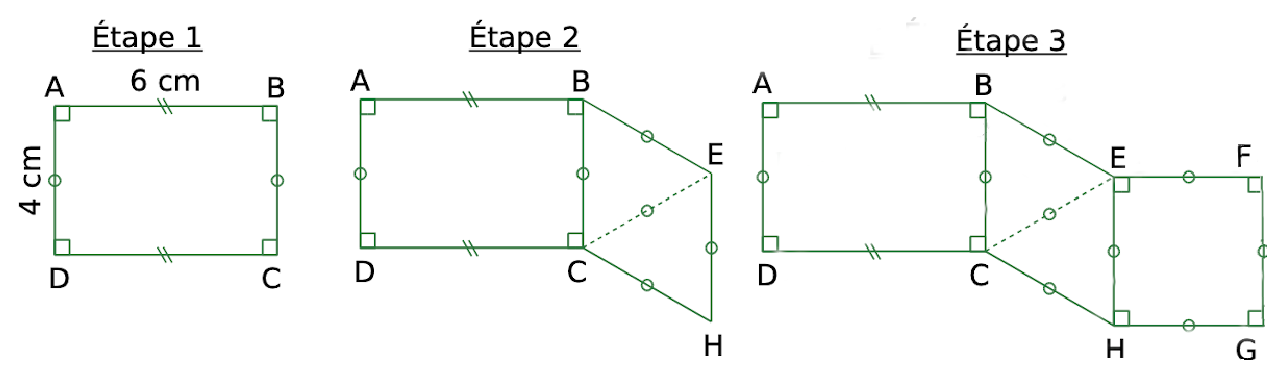
\includegraphics[width=9cm]{programme}
\end{exercice}
\hfill {\it\footnotesize Source : Sesamath, le manuel 6\up{e}. Génération 5 - 2013}
\end{colonne*exercice}


%%%%%%%%%%%%%%%%%%%%%
%%%%%%%%%%%%%%%%%%%%%
\Recreation

\enigme[Des quadrilatères dans un octogone]
   \begin{center}
   \fbox{
      \begin{minipage}{15cm}
         \parbox{5cm}{
            Tracer quatre diagonales de l'octogone régulier pour obtenir le quadrilatère demandé comme dans les exemples ci-contre.}
         \parbox{5cm}{
            \begin{pspicture}(-2.5,-2.2)(2.5,2.2)
               \pspolygon(2;22.5)(2;67.5)(2;112.5)(2;157.5)(2;-157.5)(2;-112.5)(2;-67.5)(2;-22.5)
               \psline(2;-22.5)(2;-157.5)
               \psline(2;157.5)(2;22.5)
               \psline(2;-112.5)(2;22.5)
               \psline(2;112.5)(2;-157.5)
               \pspolygon[fillstyle=solid,fillcolor=lightgray](2;-157.5)(0.32,-0.77)(2;22.5)(-1.21,0.77)
            \end{pspicture}}
         \parbox{5cm}{
            \begin{pspicture}(-2.5,-2.2)(2.5,2.2)
               \pspolygon(2;22.5)(2;67.5)(2;112.5)(2;157.5)(2;-157.5)(2;-112.5)(2;-67.5)(2;-22.5)
               \psline(2;67.5)(2;157.5)
               \psline(2;67.5)(2;-112.5)
               \psline(2;-112.5)(2;157.5)
               \psline(2;-22.5)(2;-157.5)
               \pspolygon[fillstyle=solid,fillcolor=lightgray](2;157.5)(2;67.5)(-0.32,-0.77)(-1.215,-0.77)
            \end{pspicture}}
      \end{minipage}}
   \end{center}

   {\psset{unit=0.95}
   \begin{pspicture}(-3.2,-3)(2.5,2.5)
       \pspolygon(2;22.5)(2;67.5)(2;112.5)(2;157.5)(2;-157.5)(2;-112.5)(2;-67.5)(2;-22.5)
       \rput(0,-2.5){Pour faire des essais}
    \end{pspicture}
    \begin{pspicture}(-3,-3)(2.5,2.5)
       \pspolygon(2;22.5)(2;67.5)(2;112.5)(2;157.5)(2;-157.5)(2;-112.5)(2;-67.5)(2;-22.5)
       \rput(0,-2.5){Un carré}
    \end{pspicture}
   \begin{pspicture}(-3,-3)(2.5,2.5)
       \pspolygon(2;22.5)(2;67.5)(2;112.5)(2;157.5)(2;-157.5)(2;-112.5)(2;-67.5)(2;-22.5)
       \rput(0,-2.5){Un autre carré}
   \end{pspicture}
 
   \begin{pspicture}(-3.2,-3)(2.5,2.3)
      \pspolygon(2;22.5)(2;67.5)(2;112.5)(2;157.5)(2;-157.5)(2;-112.5)(2;-67.5)(2;-22.5)
      \rput(0,-2.5){Pour faire des essais}
   \end{pspicture}
   \begin{pspicture}(-3,-3)(2.5,2.3)
      \pspolygon(2;22.5)(2;67.5)(2;112.5)(2;157.5)(2;-157.5)(2;-112.5)(2;-67.5)(2;-22.5)
      \rput(0,-2.5){Un rectangle}
   \end{pspicture}
   \begin{pspicture}(-3,-3)(2.5,2.3)
      \pspolygon(2;22.5)(2;67.5)(2;112.5)(2;157.5)(2;-157.5)(2;-112.5)(2;-67.5)(2;-22.5)
      \rput(0,-2.5){Un parallélogramme}
   \end{pspicture}

   \begin{pspicture}(-3.2,-3)(2.5,2.3)
      \pspolygon(2;22.5)(2;67.5)(2;112.5)(2;157.5)(2;-157.5)(2;-112.5)(2;-67.5)(2;-22.5)
      \rput(0,-2.5){Pour faire des essais}
   \end{pspicture}
   \begin{pspicture}(-3,-3)(2.5,2.3)
      \pspolygon(2;22.5)(2;67.5)(2;112.5)(2;157.5)(2;-157.5)(2;-112.5)(2;-67.5)(2;-22.5)
      \rput(0,-2.5){Un losange}
   \end{pspicture}
   \begin{pspicture}(-3,-3)(2.5,2.3)
      \pspolygon(2;22.5)(2;67.5)(2;112.5)(2;157.5)(2;-157.5)(2;-112.5)(2;-67.5)(2;-22.5)
      \rput(0,-2.5){Un autre losange}
  \end{pspicture}}

   \vfill\hfill{\footnotesize\it Source : inspiré de \href{http://www-irem.univ-paris13.fr/site_spip/IMG/pdf/activitepapierquad1.pdf}{Angles, parallélogrammes et programmation au cycle 4}, IREM Paris-Nord.}

